\documentclass[12pt,letterpaper]{article}
\usepackage[margin=1in]{geometry}

\usepackage[utf8]{inputenc} % OJO!!!  => MANTENER ESTA LINEA PARA FACIL CONVERSION A WORD EN EL FUTURO ...
% \usepackage[spanish]{babel}
\usepackage{graphicx} 
\usepackage{array}
\usepackage{tabularx}
\usepackage{amssymb, amsmath}

% Paquetes extras ... 
\usepackage{subfigure}
\usepackage{color}
\definecolor{mygreen}{RGB}{28,172,0} % color values Red, Green, Blue
\definecolor{mylilas}{RGB}{170,55,241}

\usepackage{hyperref}
\usepackage{enumitem}

\usepackage{amsmath,amsfonts,amssymb,amsthm,cancel,icomma,nicefrac,mathrsfs,
            eurosym,verbatim,environ,ifthen,ifdraft,pdfpages,float,booktabs}
\allowdisplaybreaks[1] 

\usepackage{color}
\definecolor{lstgrey}{rgb}{0.95,0.95,0.95}
\usepackage{listings}
\lstset{language=Matlab,
       backgroundcolor=\color{lstgrey},
       frame=single,
       basicstyle=\footnotesize\ttfamily,
       captionpos=b,
       tabsize=2,
  }

\lstset{language=Matlab,%
  %basicstyle=\color{red},
  breaklines=true,%
  morekeywords={matlab2tikz},
  keywordstyle=\color{blue},%
  morekeywords=[2]{1}, keywordstyle=[2]{\color{black}},
  identifierstyle=\color{black},%
  stringstyle=\color{mylilas},
  commentstyle=\color{mygreen},%
  showstringspaces=false,%without this there will be a symbol in the places where there is a space
  numbers=left,%
  numberstyle={\tiny \color{black}},% size of the numbers
  numbersep=9pt, % this defines how far the numbers are from the text
  emph=[1]{for,end,break},emphstyle=[1]\color{red}, %some words to emphasise
  %emph=[2]{word1,word2}, emphstyle=[2]{style},    
}

\title{Asignment 3}
\author{Jose Eduardo Laruta Espejo \\ Facultad de Ingeniería - Universidad Mayor de San Andrés}
\begin{document}
\maketitle
\section{Problem 1}
An adaptive filter has been found with LMS algorithm:
\lstinputlisting[label={lst:code1}, caption={Code for Problem 1}]{../matlab/heart_beat.m}

\subsection{Mother's BPM}
The results for the mother's BPM are 69.276 beats per minute.

\subsection{Baby's BPM estimation}

with the following results: a plot of the three waveforms can be seen in Fig \ref{fig:f1} and the filter coefficients in Fig \ref{fig:f4}
\begin{figure}[!h] 
  \centering
  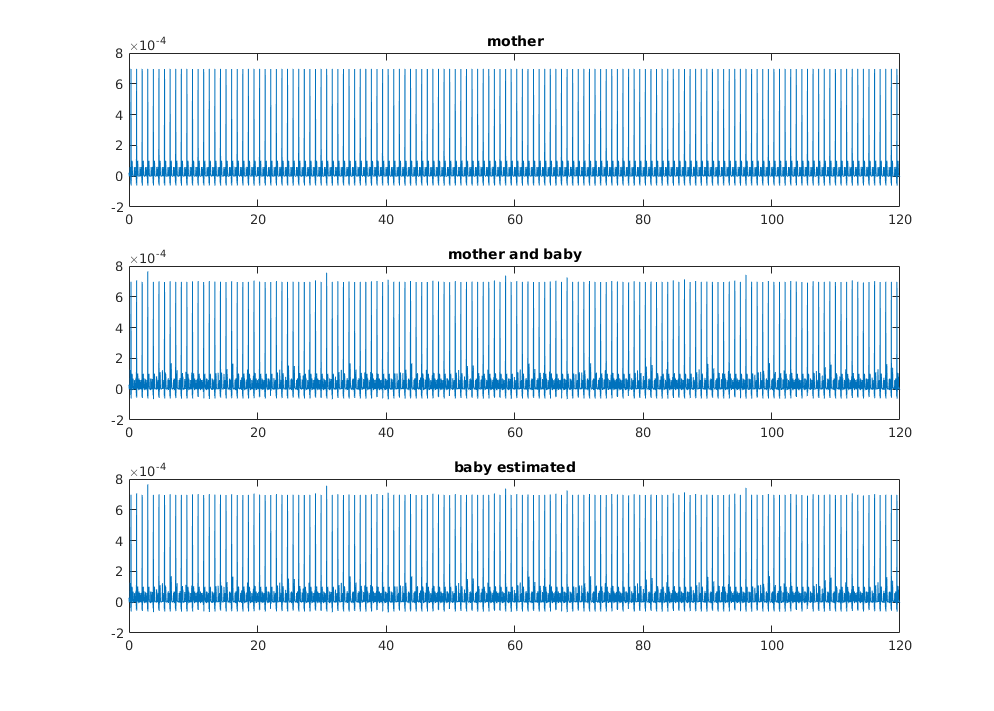
\includegraphics[width=0.8\textwidth]{../matlab/img/res.png}
  \caption{plots for heart beat estimation}
  \label{fig:res}
\end{figure}
\begin{figure}[!h] 
  \centering
  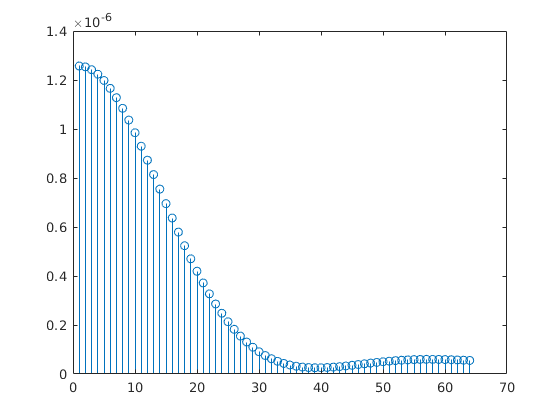
\includegraphics[width=0.8\textwidth]{../matlab/img/w.png}
  \caption{W filter coefficients}
  \label{fig:res}
\end{figure}


however, the result for the estimated BPM are exactly the same, hence, the adaptive filter used is not filtering out the mothers signal 
effectively.


\section{Problem 2}
\subsection{a}
The channel is given by: \texttt{h = [1 0 0 0]}.

\begin{figure}[!h] 
  \centering
  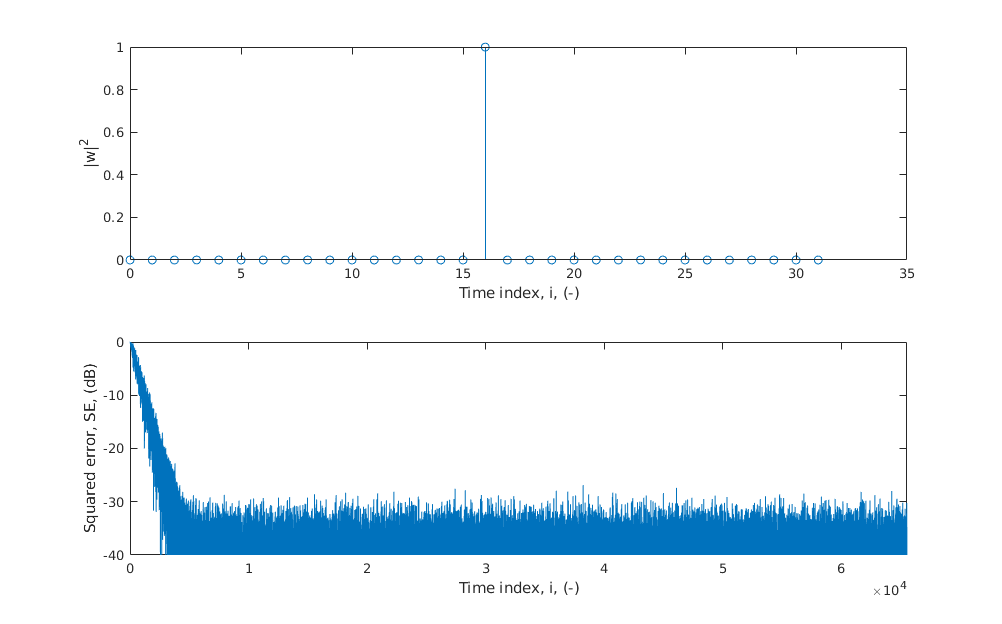
\includegraphics[width=0.8\textwidth]{../matlab/img/f1.png}
  \caption{plots for h = [1 0 0 0]}
  \label{fig:f1}
\end{figure}

\subsection{b}
The channel is given by: \texttt{h = [0 1 0 0]}.

\begin{figure}[!h] 
  \centering
  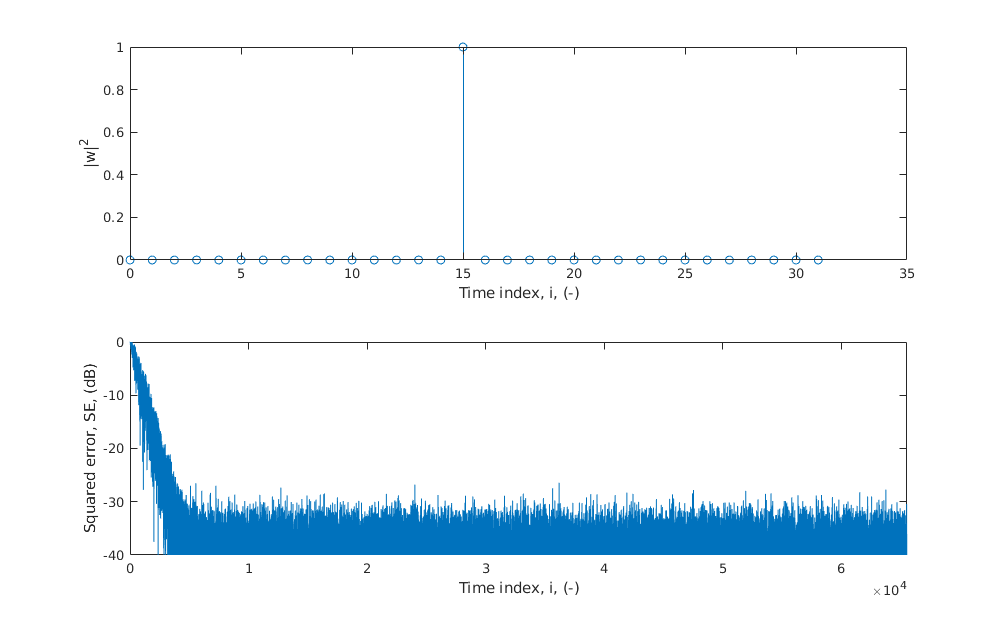
\includegraphics[width=0.8\textwidth]{../matlab/img/f2.png}
  \caption{plots for h = [0 1 0 0]}
  \label{fig:f2}
\end{figure}

The equalizer coefficients have been \textbf{shifted} one position to the left due to the corresponding shift 
in the channel filter.

\subsection{c}
The channel is given by: \texttt{h = [1 0.5 0.3 0.2]}.

\begin{figure}[!h] 
  \centering
  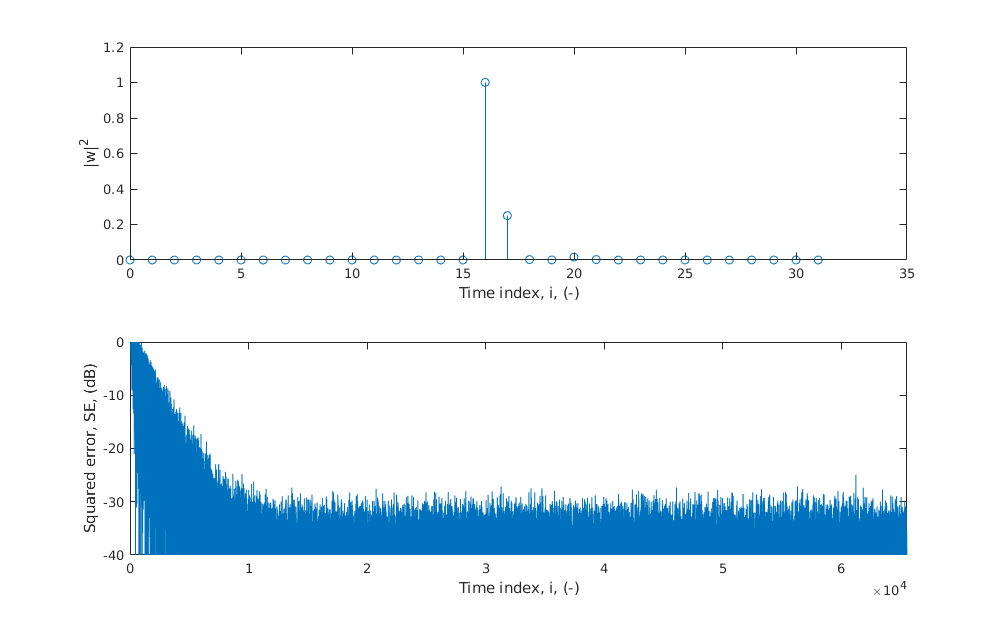
\includegraphics[width=0.8\textwidth]{../matlab/img/f3.png}
  \caption{plots for h = [1 0.5 0.3 0.2]}
  \label{fig:f3}
\end{figure}

after $\underline{w}$ converged, the convolution $\underline{h}*\underline{w}$ can be seen in Fig \ref{fig:conv}.

\begin{figure}[!h] 
  \centering
  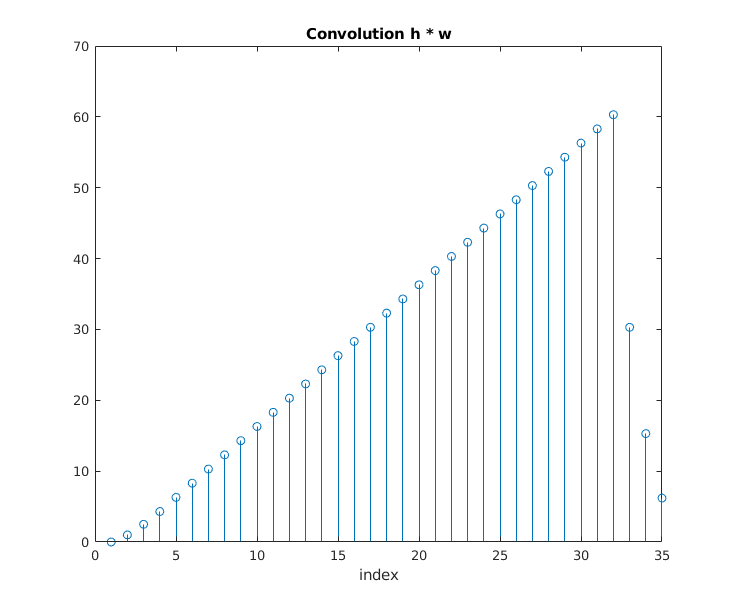
\includegraphics[width=0.8\textwidth]{../matlab/img/conv.png}
  \caption{convolution result}
  \label{fig:conv}
\end{figure}

whit this result it is reasonable to conclude that the equalizer \textbf{has undone} the channel distortion.

\subsection{d}

The channel is given by: \texttt{h = [1 1 0 0]}.

\begin{figure}[!h] 
  \centering
  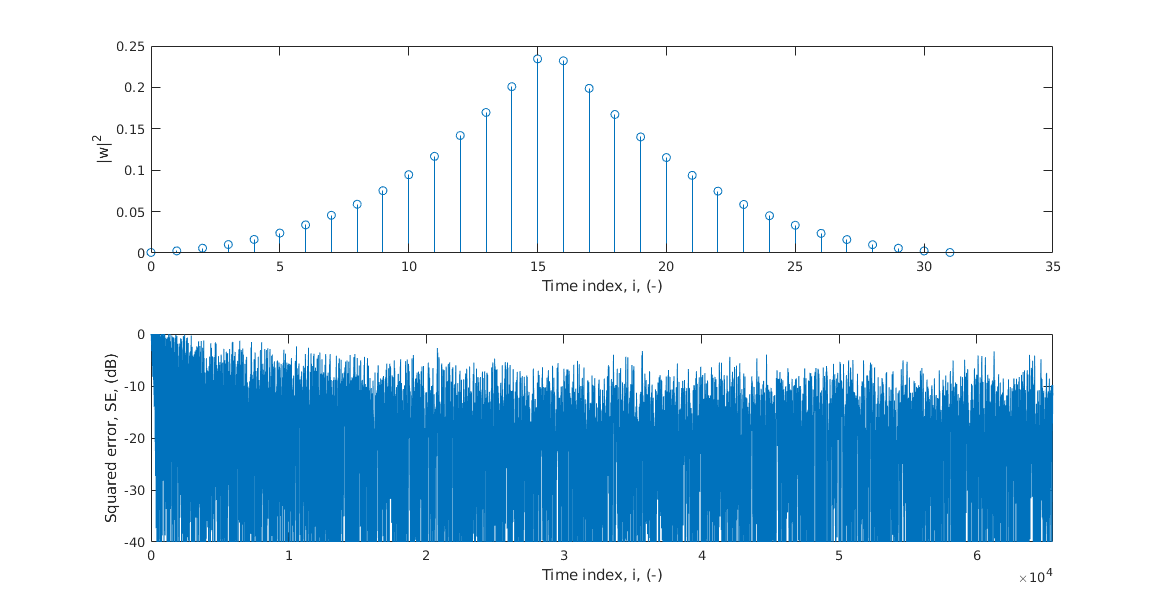
\includegraphics[width=0.8\textwidth]{../matlab/img/f4.png}
  \caption{plots for h = [1 1 0 0]}
  \label{fig:f4}
\end{figure}

after $\underline{w}$ converged, the convolution $\underline{h}*\underline{w}$ can be seen in Fig \ref{fig:conv2}.

\begin{figure}[!h] 
  \centering
  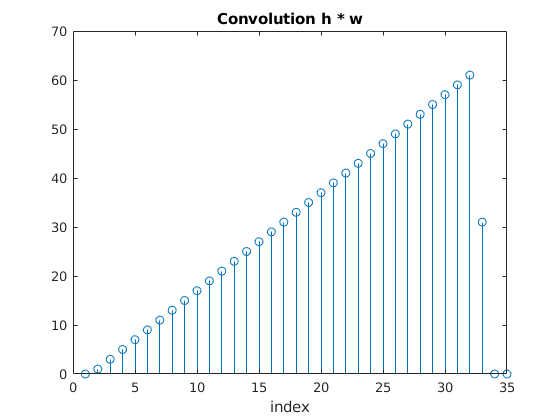
\includegraphics[width=0.8\textwidth]{../matlab/img/conv2.png}
  \caption{convolution result}
  \label{fig:conv2}
\end{figure}

\subsection{e}
In time-domain, the adaptive filter cannot undo the distortion because our channel, $\underline{h}$ is a combination of two 
equally weighted samples. This means, as the noise is a random process, this two samples will have different values 
\end{document}